\documentclass[xcolor=x11names,compress]{beamer}

\usepackage{graphicx}
\usepackage{epstopdf}
\usepackage{tikz}
\usepackage[polish]{babel}
\usepackage[utf8]{inputenc}
\usepackage[T1]{fontenc}
\usetikzlibrary{decorations.fractals}

%% Beamer Layout %%%%%%%%%%%%%%%%%%%%%%%%%%%%%%%%%%
%%  This Beamer template was created by Cameron Bracken.
%%  Anyone can freely use or modify it for any purpose
%%  without attribution.
%%
%%  Last Modified: January 9, 2009
\useoutertheme[subsection=false,shadow]{miniframes}
\useinnertheme{default}
\usefonttheme{serif}
\usepackage{palatino}

\setbeamerfont{title like}{shape=\scshape}
\setbeamerfont{frametitle}{shape=\scshape}

\setbeamercolor*{lower separation line head}{bg=DeepSkyBlue4} 
\setbeamercolor*{normal text}{fg=black,bg=white} 
\setbeamercolor*{alerted text}{fg=red} 
\setbeamercolor*{example text}{fg=black} 
\setbeamercolor*{structure}{fg=black} 
 
\setbeamercolor*{palette tertiary}{fg=black,bg=black!10} 
\setbeamercolor*{palette quaternary}{fg=black,bg=black!10} 

\renewcommand{\(}{\begin{columns}}
\renewcommand{\)}{\end{columns}}
\newcommand{\<}[1]{\begin{column}{#1}}
\renewcommand{\>}{\end{column}}
%%%%%%%%%%%%%%%%%%%%%%%%%%%%%%%%%%%%%%%%%%%%%%%%%%

\begin{document}

\section{\scshape Spis treści}
\begin{frame}
\title{Ewakuacja tunelu w warunkach pożaru}
%\subtitle{SUBTITLE}
\author{
	Jakub Rakoczy, Michał Rus\\
	{\it dr inż. Jarosław Wąs}\\
}
\date{
	\begin{tikzpicture}[decoration=Koch curve type 2] 
		\draw[DeepSkyBlue4] decorate{ decorate{ decorate{ (0,0) -- (3,0) }}}; 
	\end{tikzpicture}  
	\\
	\vspace{1cm}
	\today
}
\titlepage
\end{frame}

\begin{frame}{Spis treści}
\tableofcontents
\end{frame}

%%%%%%%%%%%%%%%%%%%%%%%%%%%%%%%%%%%%%%%%%%%%%%%%%%%%%%
%%%%%%%%%%%%%%%%%%%%%%%%%%%%%%%%%%%%%%%%%%%%%%%%%%%%%%
\section{\scshape Matematyka}

\subsection{Slajd 1}
\begin{frame}{Slajd 1}
\begin{itemize}
\item Item A
\item Item B
\begin{itemize}
\item Subitem 1
\item Subtem 2
\end{itemize}
\item Item C
\end{itemize}
\end{frame}

%%%%%%%%%%%%%%%%%%%%%%%%%%%%%%%%%%%%%%%%%%%%%%%%%%%%%%
%%%%%%%%%%%%%%%%%%%%%%%%%%%%%%%%%%%%%%%%%%%%%%%%%%%%%%
\subsection{Slajd 2}
\begin{frame}{Slajd 2}

\end{frame}
\section{\scshape Wykresy}

\subsection{Hankin-Wright}
\begin{frame}{Hankin-Wright}
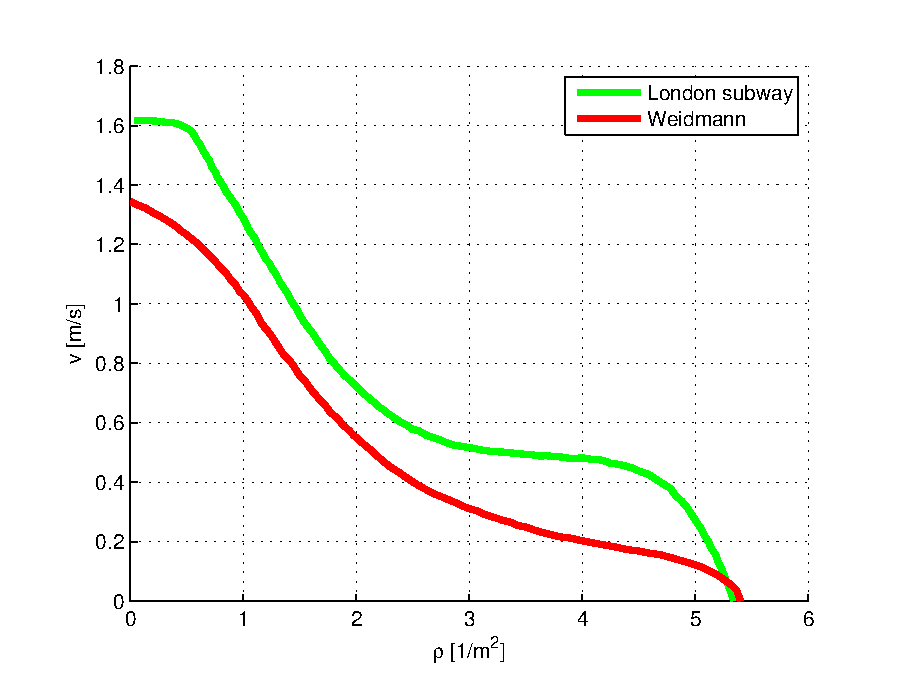
\includegraphics[width=\textwidth,height=0.8\textheight,keepaspectratio]{wykresy-hankin-wright}
\end{frame}

\subsection{Seyfried}
\begin{frame}{Seyfried}
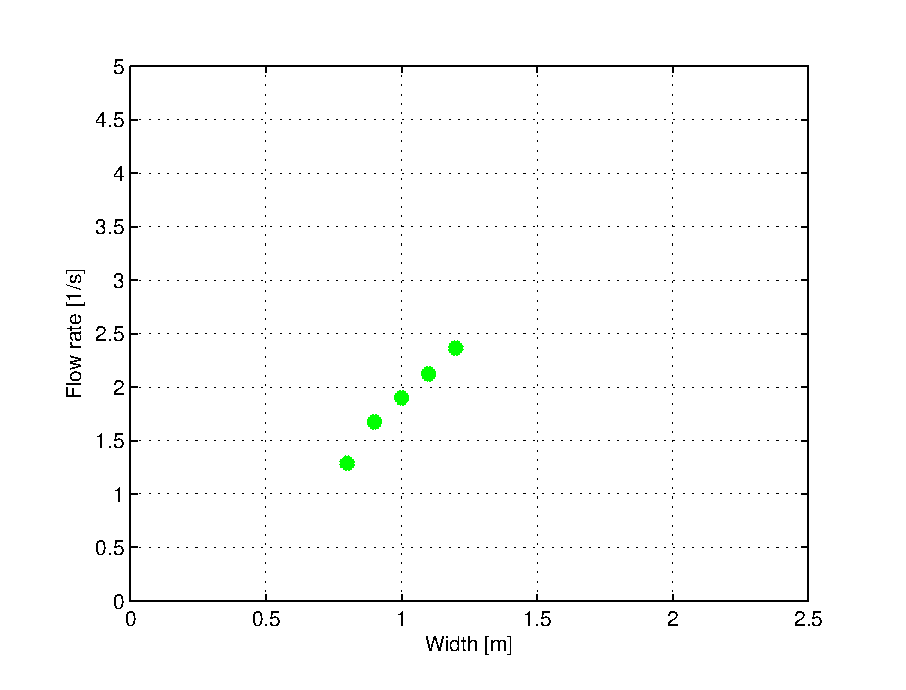
\includegraphics[width=\textwidth,height=0.8\textheight,keepaspectratio]{wykresy-seyfried}
\end{frame}

\subsection{Kuba}
\begin{frame}{Kuba}
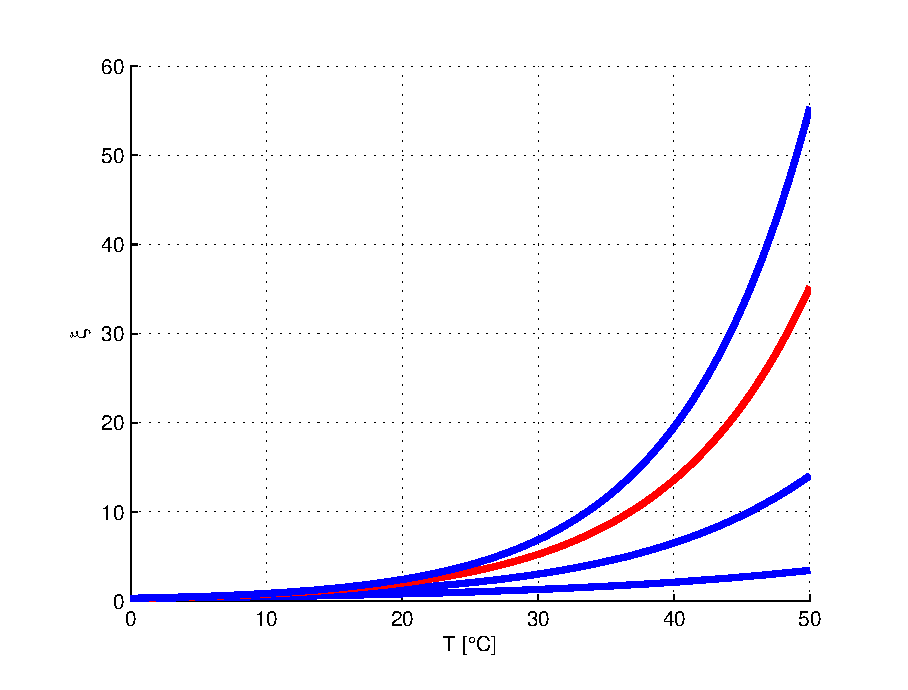
\includegraphics[width=\textwidth,height=0.8\textheight,keepaspectratio]{wykresy-kuba}
\end{frame}

\subsection{Wiki}
\begin{frame}{Wiki}
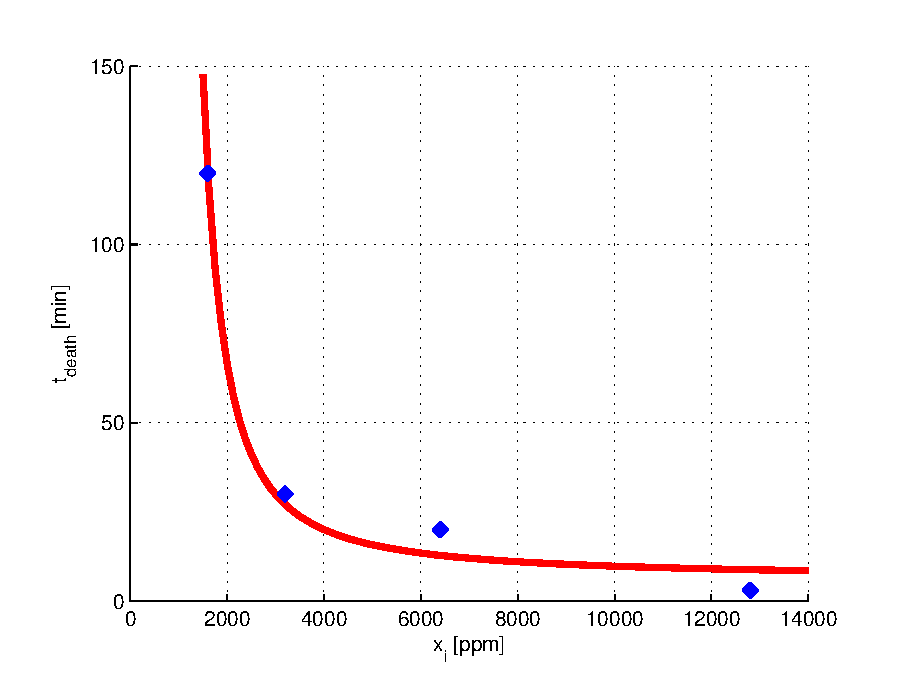
\includegraphics[width=\textwidth,height=0.8\textheight,keepaspectratio]{wykresy-wiki}
\end{frame}

\subsection{Walidacja przepływu}
\begin{frame}{Walidacja przepływu}
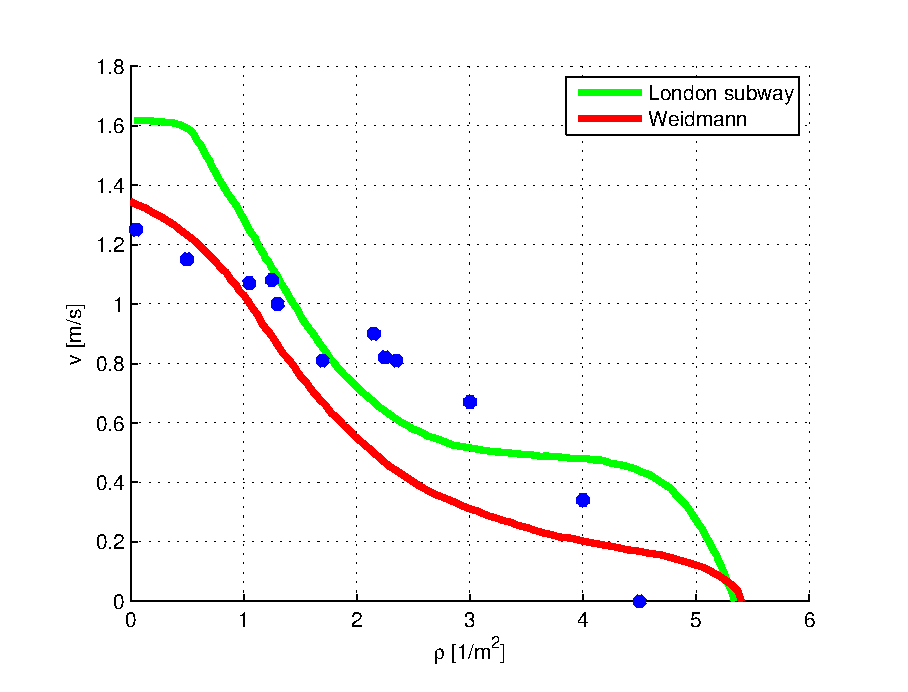
\includegraphics[width=\textwidth,height=0.8\textheight,keepaspectratio]{wykresy-weidmann_valid}
\end{frame}

\subsection{Bottleneck}
\begin{frame}{Bottleneck}

\begin{figure}
\centering
\begin{subfigure}{.5\textwidth}
  \centering
  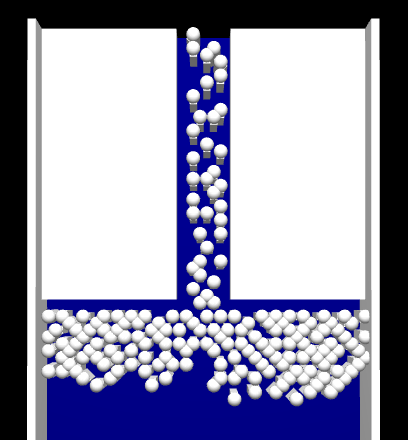
\includegraphics[width=.9\linewidth]{obrazek-bottleneck}
\end{subfigure}%
\begin{subfigure}{.5\textwidth}
  \centering
  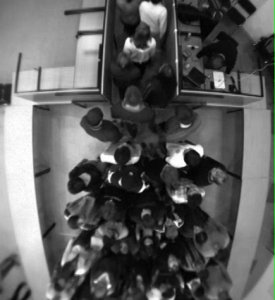
\includegraphics[width=.9\linewidth]{obrazek-bottleneck-real}
\end{subfigure}
\label{fig:test}
\end{figure}

\end{frame}

\end{document}